% Instructions to change to html version:
% Comment out:
%  minipage, multicols,columnbreak, mathbf, hrule
% Replace all: \begin{minipage}% \end{minipage} %\begin{multicols}  %\end{multicols}  %\columnbreak %% \begin{framed} %\end{framed} %%\hrule
% Replace \mathbf with \boldsymbol
% Replace $$ with \[ or \]and $ with \( or \)
% Enclose graphics in figure environments and add captions
% 			search \includegraphics
% Re-tag \df environments as sections, subsections, etc.
% Command Line Code to Create html version:
%First: pdflatex -shell-escape filename.tex                                   
%Second, for each figure: inkscape "filename-figure1.pdf" -o "filename-figure1.png"
% Third: htlatex filename.tex "ht5mjlatex.cfg, charset=utf-8" " -cunihtf -utf8"

\documentclass[10pt]{article}

%\usepackage{tikz, pgf,pgfplots,wasysym,array}
%\usepackage{wasysym,array}

\usepackage{amsmath,amssymb}

\ifdefined\HCode
  \def\pgfsysdriver{pgfsys-tex4ht-updated.def}
\fi 
%\ifdefined\HCode
%  \def\pgfsysdriver{pgfsys-dvisvgm4ht.def}
%\fi 
\usepackage{tikz}
\usetikzlibrary{calc,decorations.markings,arrows}
\usepackage{pgfplots}

\pgfplotsset{compat=1.12}
\usepackage{myexternalize}
\usetikzlibrary{calc,decorations.markings,arrows}
\usepackage{framed}
\usepackage[none]{hyphenat}

\input{../../../common/1336_header_test.tex}
\begin{document}

\everymath{\displaystyle}


\newcommand{\ihat}{\boldsymbol{\hat{\textbf{\i}}}}
\newcommand{\jhat}{\boldsymbol{\hat{\textbf{\j}}}}
\newcommand{\khat}{\boldsymbol{\hat{\textbf{k}}}}

\let\oldvec\vec
\renewcommand{\vec}[1]{\oldvec{\boldsymbol{#1}}}

\renewcommand{\u}{\vec{u}}
\renewcommand{\v}{\vec{v}}
\newcommand{\w}{\vec{w}}
\renewcommand{\r}{\vec{r}}
\renewcommand{\a}{\vec{a}}
\renewcommand{\b}{\vec{b}}

\newcommand{\<}{<}
\renewcommand{\>}{>}

\renewcommand{\myTitle}{MATH 1336: Calculus III}

\renewcommand{\mySubTitle}{Section 3.3: %Vector Functions, Space Curves, \& Arclength}%, 
%\& 
Curvature \vspace*{-.2in}}
%~\hfill Name: \underline{~~~~~~~~~~~~~~~~~~~~~~~~~~~~~~~~~~~~~~~~~~~~~~~}

\lectTitle{\vspace*{-.5in}\myTitle}{\vspace*{.1in}\mySubTitle \vspace*{-.2in}}


\setlength{\columnseprule}{0.4pt}
\setlength{\columnsep}{3em}

%\hspace*{-.8in}\begin{minipage}{1.25\textwidth}
%\begin{framed}
%\df{\textcolor{sblack}{Vector Functions, Space Curves, \& Arclength: }}~\\
%\begin{minipage}{.5\textwidth}
%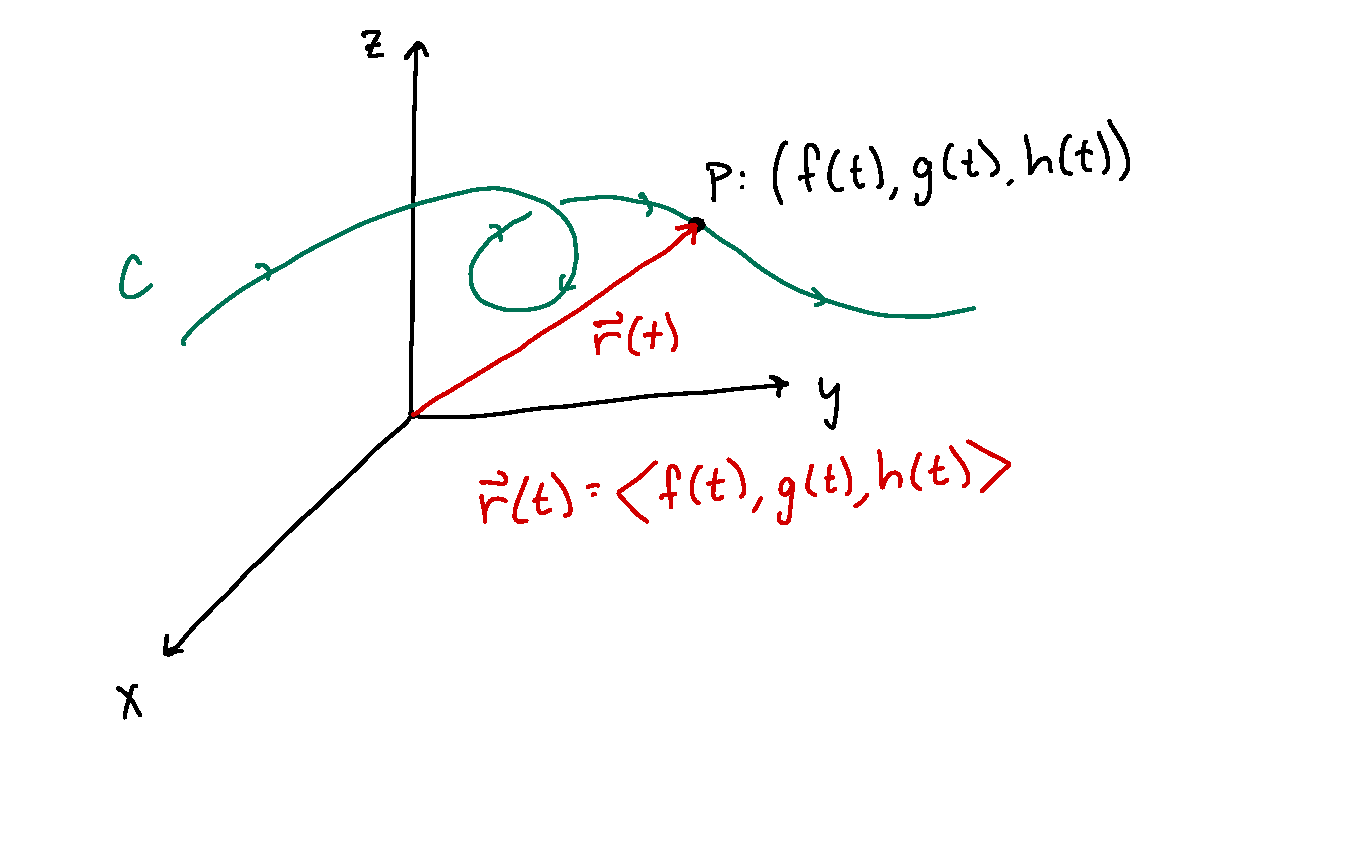
\includegraphics[width=1.1\textwidth]{Ch10s7-curve}
%\end{minipage}
%\hspace*{-.3in}
%\begin{minipage}{.5\textwidth}
%A space curve in \(\mathbb{R}^3\) can be parametrized as a \textbf{vector function} whose tip traces out the curve \(C\):
%\[
%\vec{r}(t) = \<f(t),g(t),h(t)\>
%\]
%Tangent Vector:
%\[
%\vec{r}\ '(t) = \<f'(t),g'(t),h'(t)\>
%\]
%Unit Tangent Vector:
%\[
%\vec{T}(t) = \frac{\vec{r}\ '(t)}{\Vert\vec{r}\ '(t)\Vert} 
%\]
%Definite Integrals:
%\[
%\int_a^b \vec{r}(t) dt = \<\int_a^bf(t)dt,\int_a^bg(t)dt,\int_a^bh(t)dt\>
%\]
%Arclength:
%\[
%L =\int_a^b \sqrt{\left(\frac{dx}{dt}\right)^2+\left(\frac{dy}{dt}\right)^2+\left(\frac{dz}{dt}\right)^2} dt = \int_a^b \Vert\vec{r}\ '(t)\Vert dt
%\]
%\end{minipage}
%\end{framed}
%\end{minipage}
%
%
%
%\section*{Warmup: Parallel, Perpendicular, or Neither?}
%For each of the following, determine whether the given items are parallel, perpendicular, or neither:
%\newcounter{prob}
%
%
%\begin{list}{\bf{Warmup \arabic {prob}: }}{\usecounter{prob}}
%
%%\item The vectors:
%%\[ 
%%\v_1 = < 1, 2, 3>, \qquad \v_2 = 3\ihat - 2\jhat + \frac{2}{3}\khat
%%\]
%%
%%\vfill
%%
%%\item The lines:
%%\begin{eqnarray*}
%%L_1: &\quad&  \frac{x-17}{5} = \frac{y-4}{2} = \frac{z-15}{6}\\
%%L_2: &\quad&  \frac{x+10}{6} = \frac{y+10}{4} = \frac{z+21}{9}
%%\end{eqnarray*}
%%
%%
%%\vfill
%%
%%
%\item The plane with the standard equation \(2x-y-5z = 0\) and each of the planes listed below:
%\begin{eqnarray*}
%-6x + 3y + 15z &=& 3\\
%x+2y &=& -4\\
%2x - 5z &=& -1
%\end{eqnarray*}
%
%\vfill
%
%
%\item The line with vector equation \(\r(t) = <5-3t, 2+4t, 4-2t>\) and each of the planes listed below:
%\begin{eqnarray*}
%-4.5x+6y-3z &=& -21\\
%3x + 5y - 2z &=& -30\\
%2x + 2y - 3z &=& 11\\
%4x + 7y + 8z &=& 11
%\end{eqnarray*}
%%
%%\vfill
%
%
%
%
%\end{list}
%
%\pagebreak
%
%\section*{Space Curve Examples:}
%
%%\newcounter{prob}
%
%\begin{list}{\bf{Example \arabic {prob}: }}{\usecounter{prob}}
%
%%\addtocounter{prob}{1}
%\item \textbf{We will revisit the example from the pre-class video in a Mathematica demonstration:}
%\\Answer the following question about the vector function:
%\[
%\vec{r}(t) = \< e^{2t},t^2-t,\ln t\> = e^{2t}\ \ihat + (t^2-t)\ \jhat + \ln t\ \khat
%\]
%
%\begin{enumerate}[a)]
%
%\item What is the domain of \(\vec{r}(t)\)?
%
%\vfill
%
%\item Find a tangent vector at the point where \(t=0.2\).
%
%\vfill
%
%\item Find an equation for the tangent line to \(\vec{r}(t)\) at the point where \(t=0.2\).
%
%\vfill
%
%\item What is the unit tangent vector \(\vec{T}(t)\) for \(\vec{r}(t)\)?  At \(t=0.2\)?
%
%\vfill
%
%\end{enumerate}
%
%\item Find \(\vec{r}(t)\) if \(\vec{r}\ '(t) = \< e^t, t^2, \cos 2t\>\) and \(\vec{r}(0) = \<2,1,-1\>\).
%\\
%\vfill
%
%\end{list}
%
%\section*{Space Curve Problems:}
%\begin{list}{\bf{Problem \arabic {prob}: }}{\usecounter{prob}}
%\item Calculate the length along the helix from \(t=0\) to \(t=3\pi\). Does your answer make sense? Why or why not?
%\[
%\vec{r}(t) = \<2 \cos t, 2\sin t, t\>
%\]
%
%\vfill
%
%\item For the vector function shown below, show that \(\vec{T}\ '(t) \perp \vec{T}(t)\).\\
%  (Note that this is also true in general!)
%\[
%\vec{r}(t) = t^3\ \ihat + t^6\ \jhat, \qquad t>0
%\]
%
%\vfill
%
%\item Find vector functions that represents the curves of intersection of the sphere \(x^2 + y^2 + z^2 = 4\) and the cylinder \(x^2+y^2 = 1\).
%
%\vfill

%\pagebreak
%
\section*{Curvature Examples:}

%\begin{framed}
%\begin{minipage}{.5\textwidth}
\begin{figure}[!h]
\centering
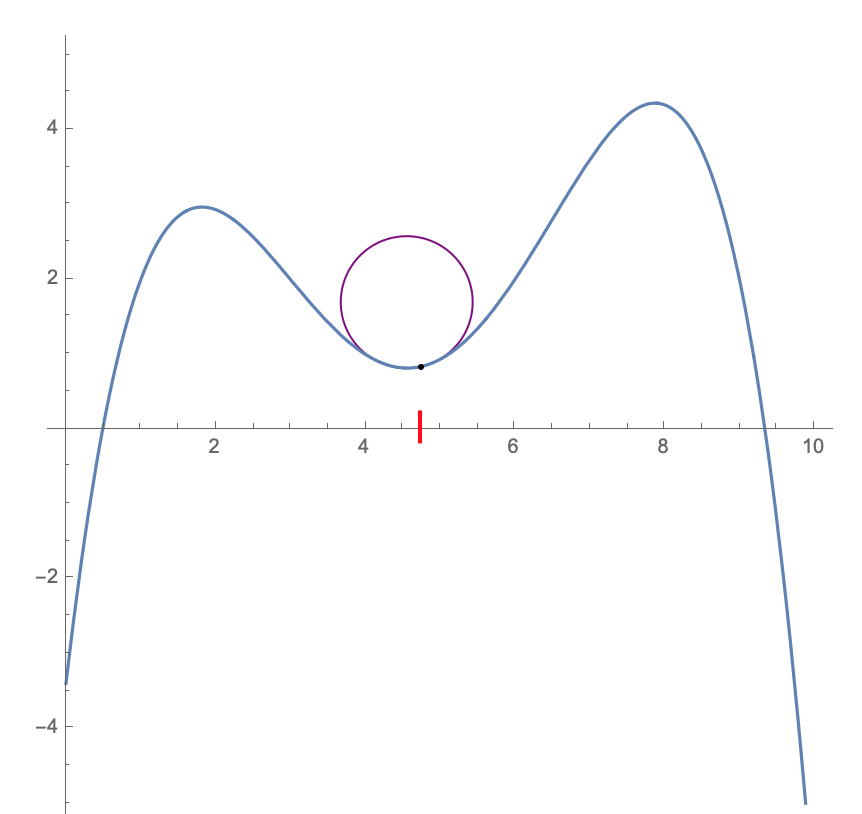
\includegraphics[width=.75\textwidth]{curvature_picture.png}
\caption{Diagram illustrating an osculating circle.}
\end{figure}
%\end{minipage}
\hspace*{-.5in}
%\begin{minipage}{.5\textwidth}
\textbf{Curvature}, denoted \(\kappa\), quantifies how quickly a curve changes direction at a given point. 
\[
\kappa = \Vert \frac{d\vec{T}}{ds}\Vert = \frac{\Vert\vec{T}\ '(t)\Vert}{\Vert\vec{r}\ '(t)\Vert} = \frac{\Vert\vec{r}\ '(t)\times \vec{r}\ ''(t)\Vert}{\Vert\vec{r}\ '(t)\Vert^3}
\]
~\\
The \textbf{osculating circle}, shown in the diagram, is the circle that is tangent to the curve at the given point and has the same curvature as the curve at that point. It has radius \(R=\frac{1}{\kappa}\).
%\end{minipage}
%\end{framed}

\newcounter{prob}
\begin{list}{\bf{Example \arabic {prob}: }}{\usecounter{prob}}

\item Show that the curvature of a line is zero!\\
Hint: the equation for a generic line is \(\vec{r}(t) = <x_0+at, y_0+bt, z_0+ct>\)

\vfill

\item Show that the curvature of the helix \(\vec{r}(t) = \<R \cos t, R \sin t, \alpha t\>\) is \(\kappa = \dfrac{R}{R^2+\alpha^2}\)
\begin{enumerate}[(a)]
\item Using the formula \(\kappa = \dfrac{\Vert\vec{T}\ '(t)\Vert}{\Vert\vec{r}\ '(t)\Vert}\)
\item Using the formula \(\kappa = \dfrac{\Vert\vec{r}\ '(t) \times \vec{r}\ ''(t)\Vert}{\Vert\vec{r}\ '(t)\Vert^3}\)
\item Which way was easier?
\end{enumerate}

\vfill
%
%\pagebreak



\end{list}

\end{document}
